%-------------------------------------------------------------------------------
%                            BAB II
%               TINJAUAN PUSTAKA DAN DASAR TEORI
%-------------------------------------------------------------------------------
\fancyhf{} 
\fancyfoot[C]{\thepage}
\chapter{TINJAUAN KEPUSTAKAAN}

\par Untuk mendukung penelitian ini, maka dalam bab ini akan dikemukakan beberapa rumusan teori pendukung, yang dikutip dari berbagai referensi baik dalam bentuk buku, artikel, maupun tulisan karya ilmiah lainnya termasuk hasil penelitian sebelumnya yang ada kaitannya dengan penelitian yang dilakukan.

\section{\textit{Indoor Positioning System}}
\textit{Indoor Positioning System} (IPS, atau \textit{"Indoor Location System"}) merupakan teknologi yang menyediakan informasi bagi pengguna berdasarkan lokasi pengguna di dalam sebuah gedung \citep{brena2017evolution}. IPS merupakan proses mendapatkan perangkat atau lokasi pengguna di dalam ruangan atau lingkungan \citep{zafari2019survey}. Banyak penelitian yang dilakukan dalam mengimplementasi IPS dengan berbagai pemanfaatan seperti WLAN. Namun pemanfaatan WLAN memiliki konsumsi daya yang boros pada smartphone sehingga pada akhirnya implementasi IPS diterapkan pada \textit{Bluetooth low Energy} (BLE) yang memiliki konsumsi daya yang lebih rendah. Metode yang dapat dilakukan dalam pengimplementasian IPS adalah metode \textit{trilateration} (berdasarkan jarak), \textit{triangulation} (berdasarkan sudut) dan \textit{fingerprinting} \citep{puspitasari2020}.

\par Pada luar ruangan untuk mendeteksi suatu lokasi sudah diterapkan dengan adanya teknologi GPS, di mana GPS banyak memberikan dampak yang luar biasa pada kehidupan sehari-hari. Namun kegunaan GPS atau sistem lokasi berbasis satelit hanya terbatas pada lingkungan di luar ruangan. Dengan demikian dibutuhkan suatu metode dan teknologi khusus untuk sistem lokasi pada dalam ruangan yang disebut sebagai \textit{Indoor Positioning System} (IPS) \citep{brena2017evolution}. Dengan menggunakan sensor dan teknologi komunikasi sistem penentuan posisi pada IPS dapat menemukan objek di lingkungan dalam ruangan. Peluang pasar pada penggunaan IPS cukup besar sehingga dapat menarik minat ilmiah komunikasi untuk menerapkan teknologi tersebut \citep{brena2017evolution}.

\par Pada teknologi IPS memiliki beberapa pendekatan yaitu, menentukan posisi dengan berbasis WiFi (WPS), menentukan posisi berbasis \textit{Bluetooth Low Energy} (BLE), menentukan posisi berbasis Identifikasi Frekuensi Radio (RFID) dan menentukan posisi dengan menggunakan teknologi \textit{Ultra-Wide Band} (UWB) atau \textit{Visible Light Communication} (VLC) \citep{canton2017bluetooth}. IPS juga dapat dipadukan dengan kemampuan \textit{route guidance} atau pemandu rute serta didampingi dengan sistem pemandu dengan suara.


\section{\textit{Route Guidance System / Wayfinding and Navigation System}}
Menurut \citep{karimi2015indoor}, \textit{Wayfinding and navigation system} memiliki 2 makna, yaitu merupakan perangkat khusus yang menyediakan solusi pencarian jalan dan navigasi tanpa memerlukan tautan komunikasi atau koneksi ke sistem lain dan tanpa penyedia pihak ketiga. Makna ke dua adalah referensi layanan melalui \textit{smartphone} yang menyediakan solusi pencarian arah dan navigasi hanya melalui tautan komunikasi kabel-nirkabel ke sistem jarak jauh yang didukung oleh penyedia pihak ketiga. Dari perspektif komputasi, \textit{Wayfinding and navigation system} adalah platform terpusat, terdistribusi, dan didistribusikan melalui klien (pada \textit{smartphone}) dan server yang dikelola oleh penyedia layanan.

\section{Kalman Filter}
Kalman Filter adalah seperangkat persamaan matematika yang menyediakan cara komputasi yang efisien untuk memperkirakan keadaan suatu proses, dengan cara meminimalkan rata-rata kesalahan kuadrat. Filter ini sangat berguna dalam beberapa aspek: mendukung estimasi-estimasi keadaan lampau, sekarang dan masa depan, dan dapat melakukannya bahkan ketika sifat pasti dari sistem yang dimodelkan tidak diketahui \cite{welch2020kalman}. Kalman Filter sendiri merupakan algoritma yang menggunakan serangkaian data yang diamati dari waktu ke waktu, yang mengandung \textit{noise} dan ketidakakuratan lainnya, untuk memperkirakan variabel yang tidak diketahui dengan lebih akurat. Ini diusulkan oleh R. E. Kalman pada tahun 1960, dan menjadi pendekatan standar untuk estimasi yang optimal. Karena memiliki keunggulan waktu secara \textit{realtime}, cepat, efisien, dan anti-interferensi yang kuat, Kalman filter telah banyak diterapkan di bidang perhitungan orbit, pelacakan target dan navigasi \cite{li2015kalman}.

\section{\textit{Fingerprinting}}
\textit{Fingerprinting} adalah teknik untuk menentukan lokasi dengan pemanfaatan \textit{Radio Signal Strength} (RSS) dari suatu \textit{Access Point }(AP). Menurut Yudha dkk. (2018) , metode ini memperhitungkan atenuasi karena kekuatan sinyal sering berubah-ubah. Setiap titik reverensi dikumpulkan yang mengintegrasikan adanya penghalang antara transmiter dan \textit{receiver}.

\par Transmiter untuk teknologi IPS yang ditunjukan untuk WLAN disebut dengan AP, sedangkan transmiter untuk teknologi IPS yang ditunjukan untuk \textit{Bluetooth Low Energy} disebut dengan \textit{Beacon } \cite{puspitasari2020}. Metode fingerprinting berbasis IPS ini terdiri dari 2 tahap. Tahap pertama adalah tahap pembelajaran (offline), di mana lokasi fingerprints itu sendiri diperoleh dengan cara mengumpulkan RSSI dalam satuan desibel (dB) yang dipancarkan dari masing-masing AP. Kemudian gelombang radio yang dipancarkan AP yang diletakkan pada posisi yang telah ditentukan sebelumnya ditangkap oleh smartphone yang terintegrasi dengan WLAN ataupun \textit{Bluetooth}.

\par Selama tahap pembelajaran lokasi yang tidak diketahui data pembelajarannya kemudian dirujuk sebagai titik referensi estimasi lokasi. Tahap kedua adalah tahap pengujian (\textit{online}), di mana keakuratan yang dikumpulkan dalam data pembelajaran. Selama tahap pengujian sistem harus memberikan lokasi setiap objek berdasarkan data RSSI yang diamati. Namun, nilai RSSI bisa dipengaruh oleh keadaan lingkungan sekitar yang dapat mengganggu keakuratannya (\citep{subhan2011indoor}). Menurut \citep{yudha2018indoor}, metode Fingerprinting berbasis IPS ini melibatkan 2 tahap yang dapat dilihat pada Gambar x.x.

\begin{figure}[H]
\centering
\shadowbox
{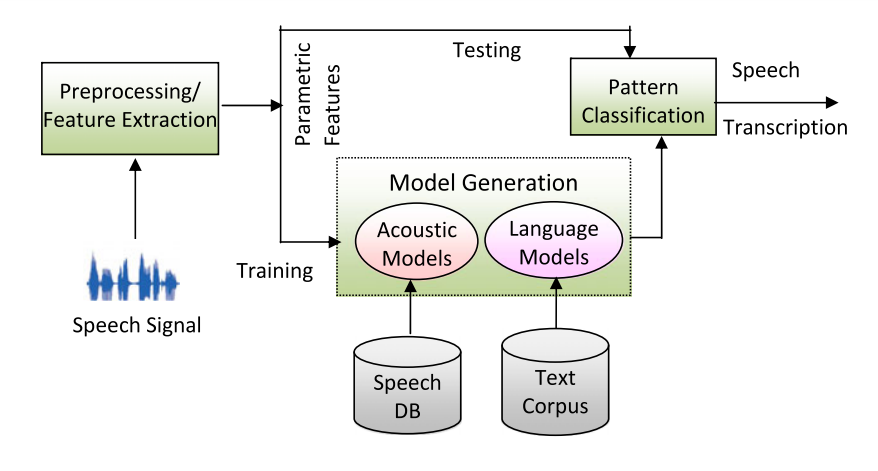
\includegraphics [width = 10cm, height= 5cm]{gambar/sr_arsitektur}}
\caption{Ilustrasi Metode \textit{Fingerprinting} \citep{aggarwal2012}}.
\label{sr_arsitektur}
\end{figure}

\section{\textit{Received Signal Strength Indicator} (RSSI)}
\textit{Received Signal Strength Indicator} atau RSSI adalah metode pengukuran jarak yang memperoleh sinyal dari transmiter seperti \textit{Bluetooth} untuk menentukan \textit{distance-loss} model, dan kemudian memperkirakan posisi pengguna melalui beberapa algoritma (\citep{li2018indoor}). Menurut \citep{puspitasari2020} \textit{Positioning System} menghasilkan data yang penting untuk menghitung lokasi pengguna. \textit{Time of Arrival} (TOA), \textit{Time Difference of Arrival} (TDOA), \textit{Angle of Arrival} (AOA). RSSI memperkirakan jarak \textit{node} yang belum diketahui ke referensi \textit{node} dari beberapa kumpulan unit perhitungan dengan menggunakan atenuasi kekuatan sinyal (\textit{signal strength}) yang dipancarkan oleh transmiter \citep{puspitasari2020}.

\par Nilai RSSI didefinisikan dengan bilangan negatif. Semakin tinggi bilangan negatifnya, maka kekuatan sinyal tersebut tergolong lemah. Namun apabila nilainya mendekati 0, maka sinyal tersebut tergolong kuat. RSSI dapat digolongkan menjadi 5 kategori kekuatan sinyal seperti pada \ref{tab:sinyal_rssi}

\begin{table}[]
\caption{Kekuatan sinyal RSSI \citep{sideeq2016smart}}
\label{tab:sinyal_rssi}
\begin{tabular}{|l|l|l|}
\hline
{\color[HTML]{000000} \textbf{No.}} & \textit{\textbf{Signal Noise Ratio }}(SNR) & \textbf{RSSI} \\ \hline
1. & Kurang dari -40 dB   & Luar Biasa  \\ \hline
2. & -40 dB hingga -55 dB & Sangat Baik \\ \hline
3. & -55 dB hingga -70 dB & Baik        \\ \hline
4. & -70 dB hingga -80 dB & Cukup Baik  \\ \hline
5. & Lebih dari -80 dB    & Buruk       \\ \hline
\end{tabular}
\end{table}

\section{\textit{Bluetooth Low Energy)} (BLE)}
Teknologi \textit{Bluetooth} dikembangkan oleh Ericsson pada tahun 1994 dengan kegunaan sebagai standar komunikasi nirkabel untuk bertukar data dalam jarak dekat \citep{kaluvza2017analysis}. Teknologi \textit{Bluetooth} memiliki fitur utama yaitu memiliki biaya yang rendah, konsumsi daya rendah, jangkauan kecil, memiliki ketahanan dan penggunaan secara global. Kecepatan transfer data yang diberikan oleh \textit{Bluetooth} sebesar 1 Mbit/s dan menggunakan pita frekuensi tanpa izin 2,4 hingga 2,485 GHz \citep{kaluvza2017analysis}.

\par Pertengahan tahun 2010 spesial otoritas kompeten yang bernama “Bluetooth Special Interest Group" (SIG) mengumumkan spesifikasi \textit{Bluetooth} 4.0, dimana meliputi : \textit{Bluetooth} Klasik, \textit{Bluetooth} dengan kecepatan tinggi, dan protokol \textit{Bluetooth} hemat energi. Karakteristik dari \textit{Bluetooth Low Energy} (BLE) adalah memiliki ukuran yang kecil, menggunakan biaya rendah, konsumsi penggunaan daya yang rendah dengan kemungkinan penggunaan sampai beberapa tahun bekerja dengan menggunakan baterai AAA dan memiliki kompatibilitas dengan perangkat seluler, tablet, dan komputer \citep{kaluvza2017analysis}.



\section{\textit{Beacon}}
BLE memancarkan sinyal dari alat transmiter yang beroperasi menggunakan baterai. Alat transmiter tersebut disebut dengan \textit{Beacon}. \textit{Beacon} merupakan alat pendeteksi lokasi dengan harga yang terjangkau, ukurannya yang kecil, memiliki daya tahan baterai yang cukup lama, dan tidak membutuhkan energi listrik tambahan \citep{puspitasari2020}. Setiap perangkat \textit{smartphone} dan tablet yang mendeteksi sinyal dari \textit{Beacon}, dapat menghitung jarak dan memperkirakan keberadaan lokasi setiap perangkat sekaligus. \textit{Beacon Bluetooth} mengubah pengalaman menggunakan \textit{smartphone} untuk bepergian, berbelanja, bekerja, dan bermain \citep{kaluvza2017analysis}.

\section{\textit{Speech Recognition}}
\textit{Speech Recognition} adalah kemampuan suatu komputer agar dapat mengenali apa yang diucapkan oleh seseorang berdasarkan sinyal suara yang diucapkan oleh seseorang atau bisa disebut sebagai \textit{Automatic Speech Recognition} (ASR)\citep{jurafskyspeech2008}. \textit{Speech Recognition} merupakan antarmuka alami untuk berkomunikasi dengan peralatan komputer seperti \textit{smart home appliances}, \textit{personal assistants}, atau \textit{smartphone}. ASR Juga berguna untuk \textit{general transcription}, contohnya untuk membuat \textit{captions} secara otomatis untuk audio atau video (mentranskripsikan film atau video atau \textit{live discussions}) (Daniel & James, 2020). Menjadi suatu kemudahan bagi manusia jika komputer dapat memahami apa yang diucapkan oleh manusia dan karena hal itu juga manusia dapat dengan mudah mengoperasikan komputer karena adanya teknologi yang \textit{Automatic Speech Recognition}. serta \textit{speech synthesis} atau \textit{text-to-speech} (TTS) \citep{jurafskyspeech2008}.

\section{\textit{Text-to-Speech }(TTS)}
Speech Syntesis atau text-to-speech merupakan kebalikan dari ASR dalam memetakan teks ke bentuk gelombang akustik. TTS memilik berbagai macam aplikasi. TTS digunakan dalam agen percakapan yang berdialog dengan orang-orang, berperan dalam perangkat yang membacakan dengan keras untuk tunanetra atau dalam permainan, dan dapat digunakan untuk berbicara bagi penderita gangguan neurologis, seperti mendiang Steven Hawking seorang ahli astrofisika berbicara dengan memanipulasi sistem TTS \citep{jurafskyspeech2008}.

\section{KALDI \textit{Toolkit}}
Kaldi adalah toolkit open-source untuk speech recognition, Kaldi ditulis dalam bahasa C++ dan di bawah lisensi Apache v2.0, Kaldi bergantung dengan library finite-state transducers (menggunakan OpenFst) serta library aljabar linier ekstensif menggunakan "Basic Linear Algebra Subroutines" (BLAS) dan "Linear Algebra PACKage" (LAPACK) \citep{povey2011}. Pada penelitian ini akan digunakan model yang dihasilkan oleh Kaldi untuk membangun model yang akan digunakan pada VOSK API.


\section{VOSK API}
Vosk api merupakan toolkit untuk speech recognition, di mana memiliki beberapa kelebihan, yaitu \citep{cephei2019}:
\begin{enumerate}
\item Memiliki 19 lebih bahasa dan dialek yang didukung vosk.
\item Vosk api merupakan toolkit speech recognition yang bisa digunakan secara offline, yang dapat digunakan pada Raspberry Pi, Android, iOS.
\item Kemudahan untuk menginstalasi vosk dengan menggunakan pip3 install vosk.
\item Model yang portabel pada masing-masing bahasa sebesar 50Mb, namun ada beberapa model server yang lebih besar pula.
\item Menyediakan streaming API untuk pengalaman pengguna terbaik.
\item Memiliki beberapa paket bahasa pemograman yang berbeda-beda, seperti java, csharp, javascript dll.
\item Untuk akurasi terbaik dapat memungkinkan konfigurasi ulang kosakata dengan cepat.
\item Mendukung identifikasi pembicara selain dengan speech recognition yang sederhana.

\end{enumerate}

\section{Android}
Android merupakan suatu \textit{software} (perangkat lunak) yang digunakan pada \textit{mobile device}(perangkat berjalan)yang meliputi sistem operasi, \textit{middleware},dan aplikasi inti. Android \textit{Standart Development Kit} (SDK) menyediakan alat dan \textit{Application Programming Interface}(API) yang diperlukan untuk memulai pengembangan aplikasi pada platform Android menggunakan bahasa pemrograman Java, yaitu kode Java yang terkompilasi dengan data dan \textit{file resources} yang dibutuhkan aplikasi dan digabungkan oleh \textit{app tools} menjadi paket Android. \textit{File} tersebut ditandai dengan ekstensi .apk. \textit{File} inilah yang didistribusikan sebagai aplikasi dan dipasang pada perangkat \textit{mobile} \citep{nasution2018perancangan}.

\par Menurut \citep{shaheen2017android}. Ada 4 jenis komponen aplikasi. Setiap jenis memiliki tujuan yang berbeda dan memiliki siklus proses yang berbeda yang menentukan bagaimana komponen di \textit{create} dan di \textit{destroy}. Berikut adalah ke 4 jenis komponen tersebut:

\begin{enumerate}
\item \textit{Activities}, merupakan sebuah \textit{activity} merepresentasikan tampilan aplikasi kepada pengguna (\textit{user interface}).
\item \textit{Service}, merupakan komponen yang berjalan pada \textit{background} untuk menjalankan operasi atau proses yang tidak memiliki \textit{user interface}.
\item \textit{Content Providers}, merupakan komponen yang menangani data antar aplikasi.
\item \textit{Broadcast Receivers}, merupakan komponen yang bertanggung jawab atas menerima serta menyampaikan informasi atau notifikasi.
\end{enumerate}

\section{Android Studio}
Android Studio merupakan \textit{Integrated Development Environtment} (IDE) untuk pengembangan platform Android. Android Studio diumumkan pada tanggal 16 Mei 2013 di Google I/O \textit{Conference}. Android Studio dapat digunakan secara gratis di bawah pengawasan Apache \textit{License} 2.0. Android Studio merupakan kolaborasi antara JetBrains dan Google. Android Studio mirip dengan Eclipse yang disertai dengan ADT \textit{Plugin} (Android \textit{Development Tools})\citep{craig2015learn}.

\par Fitur-fitur Android Studio menurut \citep{puspitasari2020} adalah sebagian berikut:
\begin{itemize}
\item Proyek berbasis pada Gradle \textit{Build}.
\item \textit{Refactory} dan perbaikan bug yang cepat.
\item \textit{Tools} baru yang bernama "Lint" diklaim dapat memonitor kecepatan, kegunaan, serta kompatibilitas aplikasi dengan cepat.
\item Mendukung Proguard and \textit{App-signing} untuk keamanan.
\item Memiliki GUI aplikasi Android lebih mudah.
\item Didukung oleh Google \textit{Cloud Platform}, sehingga lebih mudah mengintegrasi Google \textit{Cloud Messaging and Application Engine} untuk setiap aplikasi yang dikembangkan.
\end{itemize}

\section{SCRUM}
Scrum adalah \textit{development framework} di mana tim lintas-fungsi mengembangkan produk atau proyek secara berulang dan bertahap. Scrum menyusun siklus pengembangan yang disebut Sprint. Iterasi ini masing-masing tidak lebih dari empat minggu dan berlangsung satu demi satu tanpa jeda \citep{deemer2012lightweight}. Sprint memiliki durasi tetap atau sprint berakhir pada tanggal tertentu baik selesai atau belum, dan tidak pernah diperpanjang. Oleh karena itu Sprint dikatakan \textit{timeboxed} (Sutherland , 2010). Tahapan-tahapan metode Scrum menurut Schwab(2013) adalah sebagai berikut :

\begin{enumerate}
\item Dimulai dengan mengumpulkan user requirements, namun tidak harus semua requirements diharapkan harus keluar dari pemikiran pengguna di tahap awal proses pengembangan. Pengguna dapat mengubah pikiran mereka di setiap waktu selama proses pengembangan, pengguna dapat menambah fitur-fitur baru, menghapus atau memperbaharui beberapa fitur yang telah ada sebelumnya.

\item Tahapan selanjutnya adalah memprioritaskan requirements dan Product Backlog. Sebuah perencanaan yang tepat dalam Sprint harus dilakukan sesuai dengan jumlah Sprint yang dibutuhkan untuk mengembangkan perangkat lunak, yang terdiri dari durasi Sprint tersebut dan requirements apa saja yang terdapat di Product Backlog yang harus diimplementasikan di setiap Sprint (dikenal dengan Sprint Backlog).

\item Sprint diawali dengan Sprint Planning di mana Product Owner, satu orang uang telah diberikan wewenang dan bertanggung jawab untuk memaksimalkan nilai produk di pasar, bertemu dengan tim Scrum (tim dengan jumlah 2-9 orang), kemudian bekerja sama untuk memperkirakan requirements dari Product Backlog apa saja yang dikerjakan selama satu Sprint.

\item Sprint Planning difasilitasi dengan Scrum Master. Scrum Master adalah seorang pemimpin yang melayani (Servant Leader). Sprint Planning memiliki batasan waktu selama 8 jam di dalam sebuah Sprint yang berdurasi selama 30 hari. Keluaran dari Sprint Planning adalah daftar pekerjaan dari hasil kesepakatan antara Product Owner dan tim Scrum di mana pekerjaan itu yang dikerjakan oleh tim Scrum nantinya selama satu Sprint beserta Sprint Goal yang dinamakan dengan Sprint Backlog.

\item Setelah Sprint Planning berakhir, tim Scrum akan mengambil Sprint Backlog untuk diri mereka masing-masing dan mengerjakan Sprint Backlog setiap hari hingga akhir Sprint tanpa campur tangan dari pihak mana pun. Daily Scrum akan dikerjakan oleh tim Scrum yang tidak lebih dari 15 menit untuk menentukan apa saja yang akan mereka kerjakan selama 24 jam ke depan berdasarkan perkembangan 24 jam terakhir, serta menyampaikan permasalahan yang menghambat mereka untuk bisa mencapai Sprint Goal. Tim Scrum akan melakukan perbaikan-perbaikan item dari Product Backlog pada Sprint yang akan datang selama proses pengembangan berlangsung, dengan tujuan membuat Sprint Planning menjadi lebih efektif.

\item Di akhir Sprint saat acara Sprint Review, Product Owner akan mempresentasikan hasil pekerjaan tim Scrum selama satu Sprint dan juga menjelaskan apa saja pencapaian tim Scrum menuju Sprint Goal di dalam Sprint tersebut kepada para pemegang kepentingan (stakeholder) agar mendapatkan feedback. Feedback ini akan dimasukkan ke dalam Product Backlog agar meningkatkan nilai dari sebuah produk. Sprint Review memiliki batasan waktu tidak lebih dari 4 jam untuk sprint yang memiliki durasi selama 30 hari.

\item Setelah Sprint Review, Scrum Master memfasilitasi acara yang bernama Sprint Retrospectives agar tim Scrum, Product Owner bekerja sama menentukan apa saja peningkatan yang akan mereka implementasikan di Sprint berikutnya. Definition of Done adalah salah satu hal yang ditekankan oleh tim Scrum pada saat Sprint Retrospectives.

\item Sprint Retrospectives merupakan acara yang paling penting dalam Scrum dikarenakan sifatnya yang menekankan continuous learning yang dapat meningkatkan tingkat agility perusahaan. Sprint Review memiliki batasan waktu tidak lebih dari 3 jam untuk Sprint yang memiliki durasi selama 30 hari. Setelah Sprint Retrospectives berakhir, maka Sprint berikutnya akan langsung dilakukan tanpa jeda antar Sprint. Pada setiap Sprint, Product Owner akan memastikan agar produk mencapai nilai setinggi mungkin saat pengembangan produk diakhiri. Product Owner, Scrum Master dan tim Scrum memegang komitmen, keberanian, saling menghargai satu sama lain, keterbukaan dan fokus. Ilustrasi tahapan-tahapan metode Scrum dapat dilihat pada Gambar x.x di bawah ini.
\end{enumerate}

\begin{figure}[H]
\centering
\shadowbox
{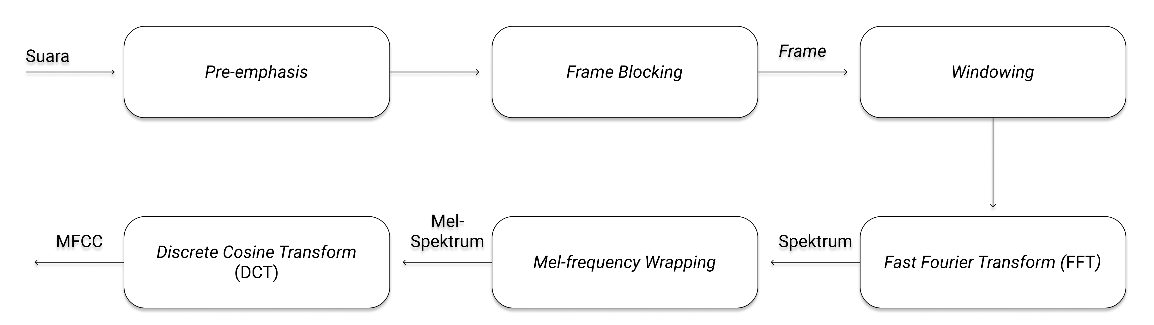
\includegraphics [width = 14cm, height= 5cm]{gambar/alir_mfcc}}
\caption{gIlustrasi Metode Pengembangan Menggunakan Scrum (Schwab, 2013).}}.
\label{alir_mfcc}
\end{figure}

\section{\textit{Black Box Testing}}
Salah satu jenis pengujian fungsional adalah blackbox testing. Blackbox testing merupakan suatu pengujian yang tidak menggunakan pengetahuan tentang struktur interior aplikasi. Saat melakukan pengujian, penguji akan berinteraksi langsung dengan user interface, lalu penguji akan memberikan masukan dan memeriksa hasil dari aplikasi yang digunakan tanpa mengetahui bagaimana proses dari hasil tersebut (Xu, Chen, Wang, dan Rud, 2016). Pada blackbox testing mendapatkan pengujian dari deskripsi eksternal perangkat lunak, termasuk spesifikasi, persyaratan, dan desain (Ammann dan Offutt, 2017).

\par Blackbox testing memiliki beberapa keuntungan, di antaranya penguji tidak perlu mengetahui suatu bahasa pemrograman, pengujian dilakukan dari sudut pandang pengguna agar dapat mengetahui suatu inkonsisten pada spesifikasi kebutuhan serta yang terakhir programmer dan penguji dapat saling bergantung (Jaya, 2018). Blackbox testing juga memiliki beberapa kekurangan yaitu suatu pengujian sulit didesain tanpa spesifikasi yang jelas, memiliki kemungkinan untuk pengulangan testing dan tidak ada pengujian pada bagian back end (Jaya, 2018).

\section{\textit{Usability Testing}}
Usability Testing adalah kegiatan pengujian untuk mengumpulkan data mengenai sebuah produk dalam tahap pengembangan. Tujuan utama dari usability testing adalah untuk mengumpulkan data kuantitatif dengan mengukur waktu untuk mengidentifikasi dan memperbaiki kekurangan yang ada dalam produk serta bahan pendukung yang menyertainya sebelum produk dirilis (Rubin dkk., 2008). Dengan usability testing, didapati apa yang sebenarnya dilakukan pengguna, apa yang berhasil untuk mereka, dan apa yang tidak dipikirkan akan mereka lakukan atau bahkan apa yang mereka pikir akan mereka lakukan jika menggunakan produk (Barnum, 2020).


\par Pengujian ini diharapkan akan mendapatkan kekuatan dan kelemahan dari setiap aspek yang ada pada aplikasi itu sendiri. Maka dari itu, perlu adanya dokumentasi pengalaman aktual para calon pengguna aplikasi atau produk saat dievaluasi (Wesfix, 2017). Tujuan lain dilakukannya pengujian ini adalah untuk mengumpilkan data kualitatif yang berhubungan dengan produk yang diuji. Data kualitatif tersebut terdiri dari komentar yang dibuat oleh partisipan, jawaban dari kuesioner pertanyaan dan tanggapan dari partisipan saat proses wawancara. Usability testing telah terbukti dapat mengurangi waktu pada tahap pengembangan, mengurangi jumlah bugs, dan menghasilkan produk yang lebih berkualitas untuk meningkatkan nilai jual (Wahl, 2000).


\section{\textit{System Usability Scale }(SUS)}
Kuesioner standar yang paling sering digunakan untuk penilaian suatu kegunaan merupakan System Usability Scale (SUS). Dari awal kuesioner ini relatif tidak menguntungkan, namun dimasa depan kemungkinan besar SUS akan menjadi suatu ukuran yang populer dari persepsi kegunaan. Mendapatkan nilai pada SUS cukup rumit, karena pola pada item yang bergantian dan memiliki keputusan awal untuk memanipulasi skor berada di antara 0 sampai 100 (Lewis, 2018). John Brooke mengembangkan SUS pada tahun 1996 yang berisi 10 pertanyaan dasar dan sederhana tentang kegunaan suatu sistem, berikut adalah pertanyaannya  (Kaya, Ozturk, dan Gumussoy, 2019):
\begin{center}
\begin{tabular}{ |c|c| } 
 \hline
 R1 & Saya pikir saya ingin menggunakan sistem ini dengan sering.\\
 R2 & Saya menemukan sistem yang tidak rumit.\\
 R3 & Saya pikir sistemnya mudah digunakan.\\
 R4 & Saya pikir saya akan membutuhkan bantuan dari orang teknis untuk dapat menggunakan sistem ini.\\
 R5 & Saya menemukan berbagai fungsi dalam sistem ini terintegrasi dengan baik.\\
 R6 & Saya pikir ada terlalu banyak inkonsistensi dalam sistem ini.\\
 R7 & Saya membayangkan bahwa kebanyakan orang akan belajar menggunakan sistem ini dengan sangat cepat.\\
 R8 & Menurut saya sistem ini sangat rumit untuk digunakan.\\
 R9 & Saya merasa sangat percaya diri menggunakan sistem ini.\\
 R10 & Saya perlu belajar banyak hal sebelum saya bisa menggunakan sistem ini.\\
 \hline
\end{tabular}
\end{center}

\par Pertanyaan tersebut akan diberikan kepada peserta uji dan menjawab dengan skala antara 1 (Sangat tidak setuju) dan 5 (Sangat setuju). Menurut Brooke hasil dari jawaban akan dievaluasi dalam kisaran 0 sampai 4. Dapat dilihat pada pertanyaan yang memiliki nomor ganjil maka memiliki makna positif dan pertanyaan bernomor genap memiliki makna negatif. Pada pertanyaan positif dilakukan penilaian yang mana skor pengguna dikurangi 1 poin dan pada pertanyaan negatif dilakukan penilaian yang mana skor pengguna dikurangi 5 poin. Setelah itu jumlah skor yang didapat dikalikan 2,5 untuk membuat kisaran antar 0 sampai 100. Skor SUS rata-rata dan skala peringkat kata sifat dihitung untuk setiap aplikasi seluler di Android dan iOS (Kaya, Ozturk, dan Gumussoy, 2019).


%-----------------------------------------------------------------------------%

% Baris ini digunakan untuk membantu dalam melakukan sitasi
% Karena diapit dengan comment, maka baris ini akan diabaikan
% oleh compiler LaTeX.
\begin{comment}
\bibliography{daftar-pustaka}
\end{comment}
